\documentclass[12pt]{article}

%% preamble: Keep it clean; only include those you need
\usepackage{amsmath}
\usepackage[margin = 1in]{geometry}
\usepackage{graphicx}
\usepackage{booktabs}
\usepackage{natbib}
% for space filling
\usepackage{lipsum}
% highlighting hyper links
\usepackage[colorlinks=true, citecolor=blue]{hyperref}
\usepackage{tabularx}
\usepackage{adjustbox}
\usepackage{booktabs}
\usepackage{multirow}
\usepackage{threeparttable}

% double spacing
\usepackage{setspace}
\doublespacing


%% meta data

\title{Bridging Gaps: Investigating COVID-19's Influence on Health Disparities in Connecticut}
\author{Delia Lin\\
  Department of Statistics\\
  University of Connecticut
}

\begin{document}
\maketitle

\begin{abstract}
  Social determinants of health (SDoH) are the conditions in which people are born, 
  grow, live, work, and age, significantly influencing their overall health and well-being. 
  These determinants include socioeconomic status, education, access to healthcare, and the 
  physical environment. Understanding the interactions of these elements will be essential for 
  addressing health disparities and developing more effective public health policies and interventions.
\end{abstract}

\section{Introduction}\label{sec:intro}
\\
I. Prevalence of Social Determinants of Health 
\\
Current research focuses on how social determinants of health (SDoH) plays a  massive
impact on one's health; it is estimated that 80 percent of a population's health outcomes are 
dictated by SDoH \citep{HOOD2016129}. Often, SDoH, when referring to an individual, can result in racial 
disparities in care when looking at a population\citep{Monroe2023-uq}. It has been shown that major inefficiencies
in the health system are attributed to overlooked prevention opportunities and unequal access
to care.\citep{Allin2014-xn}

Understanding the intricate interplay of these social determinants is crucial in addressing health disparities 
and developing effective public health policies and interventions. The COVID-19 pandemic has shed new light on 
these disparities, amplifying existing inequalities within various communities. This research topic gains paramount 
importance in the current context as it seeks to delve into the specific impact of COVID-19 on key social determinants 
of health in different counties and racial groups in Connecticut.

The existing literature underscores the pressing need for research in this area. Studies have shown that predominantly 
black counties in the United States experience significantly higher COVID-19 infection and mortality rates, emphasizing 
the racial disparities prevalent in healthcare outcomes. The pandemic has magnified these discrepancies, leading to 
mortality rates among historically marginalized minority communities that are 1.9 to 2.4 times higher compared to the 
general population \citep{Badalov2022-wt}. Additionally, inefficiencies in the healthcare system have been attributed 
to overlooked prevention opportunities and unequal access to care, necessitating a comprehensive examination 
of these social determinants in the context of the pandemic.

Despite the growing body of research on SDoH, there is a notable gap concerning the specific impact of COVID-19 on 
these determinants within diverse communities. This research aims to bridge this gap by comprehensively assessing how 
the pandemic has influenced key social determinants of health across the 8 CT counties and a four year timeframe prior to 
the start of the COVID pandemic. 
By identifying the specific ways in which different communities were affected, this study contributes valuable insights 
for targeted interventions, policy-making, and the development of equitable healthcare strategies.
\\
II. Introduction to the Impact of Social Needs(specify for CT)
\\
This study will compare each of the following social needs by Year(2017-2020) and by 8 CT Counties: 
Median Income,
Educaation,
Food Access
Housing Stability,
Health Insurance,
Reshospitalization rates.

Income is a fundamental
social need that significantly influences
one's health. The level of income
directly affects an individual's access
to essential resources such as nutritious
food, healthcare, and secure housing.
People with lower incomes often face
barriers to healthcare services and
struggle to afford a balanced diet,
leading to higher risks of chronic
illnesses. Income disparities contribute
to inequalities in health outcomes, as
those with limited financial resources
may experience higher stress levels and
reduced access to preventive care.
Addressing income inequality is crucial
for promoting overall well-being and
reducing health disparities in communities.

Education is a key social determinant
of health, influencing various aspects
of an individual's life. Higher levels
of education are associated with better
health outcomes, as education enhances
one's ability to make informed decisions
about lifestyle choices, healthcare
utilization, and disease prevention.
Limited educational opportunities can
result in lower health literacy, reducing
an individual's capacity to navigate
complex healthcare systems and understand
preventive measures. Educational
disparities contribute to a cycle of
poor health outcomes, as individuals
with lower levels of education may face
challenges in securing stable employment
and accessing adequate healthcare
resources. Addressing educational
inequalities is essential for fostering
a healthier and more equitable society.

Access to nutritious and sufficient
food is a critical social need that
directly impacts health. Food insecurity,
often linked to low income, can lead to
malnutrition, obesity, and various health
issues. Lack of access to fresh and
healthy foods contributes to the prevalence
of chronic conditions such as diabetes
and cardiovascular diseases. Current
issues related to food include disparities
in food availability, affordability, and
nutritional quality, disproportionately
affecting marginalized communities.
Addressing these issues involves promoting
food equity, supporting local agriculture,
and implementing policies that ensure
everyone has access to nutritious food,
ultimately improving overall public health.

Housing plays a vital role in determining
health outcomes. Inadequate or unstable
housing conditions can lead to physical
and mental health issues. Homelessness
and substandard living conditions expose
individuals to environmental hazards,
increase stress levels, and contribute
to the spread of infectious diseases.
The current housing crisis in many regions
exacerbates these issues, with rising
costs and limited affordable housing
options. Addressing housing as a social
need involves implementing policies to
ensure affordable housing, preventing
homelessness, and improving living
conditions to create a foundation for
better health outcomes.

Access to healthcare through insurance
is a critical social need that significantly
impacts health outcomes. Lack of health
insurance can lead to delayed or forgone
medical care, resulting in the progression
of illnesses and poorer health.
Disparities in insurance coverage contribute
to inequalities in healthcare access and
health outcomes. Current issues include
the high costs of healthcare and the
existence of uninsured or underinsured
populations. Addressing these challenges
involves expanding access to affordable
health insurance, implementing healthcare
reforms, and promoting policies that
ensure comprehensive coverage for all
individuals.

Rehospitalization refers to the phenomenon
where individuals experience repeated
hospital admissions, often due to
complications or inadequate follow-up care.
High rates of rehospitalization indicate
gaps in healthcare delivery and management,
impacting both individual well-being and
healthcare system efficiency. This social
need is indicative of issues such as
insufficient post-discharge support,
medication management, and coordination
of care. Repeated hospitalizations not
only strain healthcare resources but also
have significant implications for the
individuals involved, leading to increased
morbidity, reduced quality of life, and
higher healthcare costs. Addressing
rehospitalization requires improvements
in transitional care, enhanced coordination
among healthcare providers, and better
support systems for patients, especially
those with chronic conditions, to ensure
a smoother recovery and reduce the burden
on healthcare systems. Recognizing and
addressing these factors can contribute
to overall health improvement, prevent
unnecessary healthcare utilization, and
enhance the effectiveness of healthcare
services.

% roadmap
The rest of the paper is organized as follows.

- The data will be presented in Section\ref{sec:data}

- The methods are described in Section\ref{sec:meth}

- The results are reported in Section\ref{sec:resu}

- A discussion concludes in Section ref{sec:disc}

\section{Data}\label{sec:data}

Data was collected from The Agency for Healthcare Research and Quality (AHRQ).The dataset comprises 7 variables 
spanning a period of 4 years (2017, 2018, 2019, 2020) with observations across the 8 counties(Fairfield County, Hartford County, 
Litchfield County, Middlesex County, New Haven County, New London County, Tolland County, Windham County) in Connecticut. These variables 
encompass a total of 56 observations. The variables questions include housing, education level, income, insurance,
rehospitalization rates, food stamps usage, and population racial characteristics. The dataset includes a range of 
calculated percentages, median values, and raw observations, providing a holistic view of various factors affecting 
the communities in these counties. 

\section{Methods}\label{sec:meth}

In this study, descriptive statistics is utilized to outline the total population, racial composition, 
and education levels across the 8 counties in Connecticut. ANOVA analyses were 
conducted to assess the significance of the difference of the variables of median income, health insurance, food access, housing, and rehospitalization rates between counties and across the four years. Additional 
Tukey's HSD tests were conducted to determine the specific counties and years that have had significant differences within 
each of the variables for each county.

\section{Results}\label{sec:resu}

County names are assigned to a respective county number: 
1	Fairfield County,
2	Hartford County,
3	Litchfield County,
4	Middlesex County,
5	New Haven County,
6	New London County,
7	Tolland County,
8	Windham County.

The racial and ethnic distribution of the population of the 8 counties investigated in this study is displayed in the following graphs:
\ref{tab:Demographics1}
\ref{tab:Demographics2}


\begin{table}[h]
\label{tab:Demographics1}
  \caption{Demographics and Education Levels for Counties 1-4}
  \resizebox{\columnwidth}{!}{%
  \begin{tabular}{lccccc}
    \toprule
    \textbf{Category} & \textbf{Fairfield County} & \textbf{Hartford County} & \textbf{Litchfield County} & \textbf{Middlesex County} \\
    \midrule
    Total Population & 944,977 & 894,465.25 & 182,657.5 & 163,318.25 \\
    Race (Percent) & & & & \\
    \quad American Indian and Alaska Native & 0.24 & 0.3075 & 0.2025 & 0.195 \\
    \quad Asian & 5.2925 & 5.2925 & 1.9 & 3.0625 \\
    \quad Black or African American & 11.405 & 13.7025 & 1.83 & 5.385 \\
    \quad Native Hawaiian and Pacific Islander & 0.055 & 0.035 & 0 & 0.005 \\
    \quad White & 72.6325 & 70.67 & 92.6025 & 88.0875 \\
    Ethnicity (Percent) & & & & \\
    \quad Hispanic & 19.53 & 17.8275 & 6.15 & 6.12 \\
    \bottomrule
  \end{tabular}%
  }
\end{table}

\begin{table}[h]
  \label{tab:Demographics2}
  \caption{Demographics and Education Levels for Counties 5-8}
  \resizebox{\columnwidth}{!}{%
  \begin{tabular}{lcccc}
    \toprule
    \textbf{Category} & \textbf{New Haven County} & \textbf{New London County} & \textbf{Tolland County} & \textbf{Windham County} \\
    \midrule
    Total Population & 858,678 & 268,477.75 & 151,218.75 & 116,608.75 \\
    Race (Percent) & & & & \\
    \quad American Indian and Alaska Native & 0.1725 & 0.605 & 0.05 & 0.565 \\
    \quad Asian & 4.005 & 4.12 & 4.675 & 1.3675 \\
    \quad Black or African American & 13.34 & 5.8175 & 3.1075 & 2.33 \\
    \quad Native Hawaiian and Pacific Islander & 0.0225 & 0.025 & 0 & 0.015 \\
    \quad White & 73.2875 & 80.6175 & 88.025 & 88.8725 \\
    Ethnicity (Percent) & & & & \\
    \quad Hispanic & 17.885 & 10.5 & 5.4475 & 11.6375 \\
    \bottomrule
  \end{tabular}%
  }
\end{table}

\begin{figure}[tbp]
  \label{fig:Education by County Graph}
    \centering
    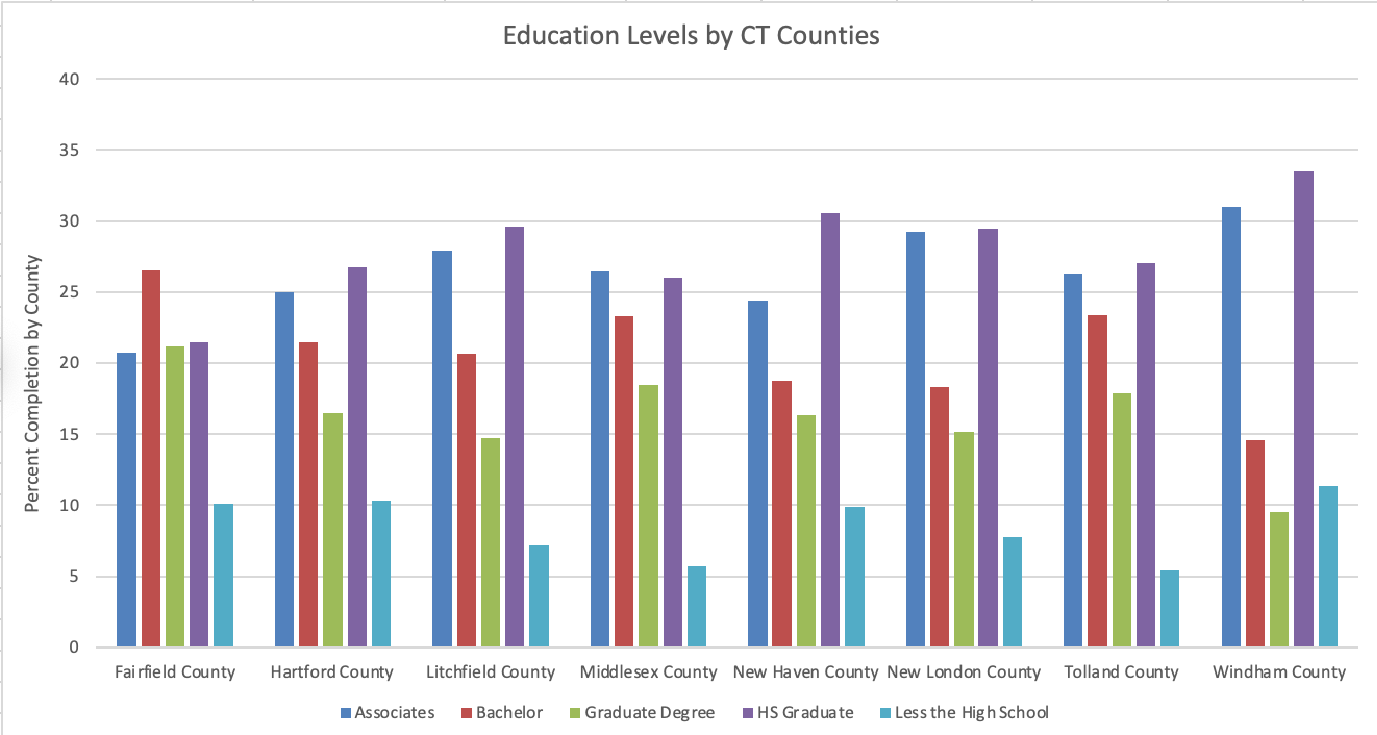
\includegraphics[width=\textwidth]{Education Levels by County.pdf}
    \caption{Education Levels by County.}
  \end{figure}


\begin{figure}[tbp]
  \label{fig:Social Needs by County Graph}
    \centering
    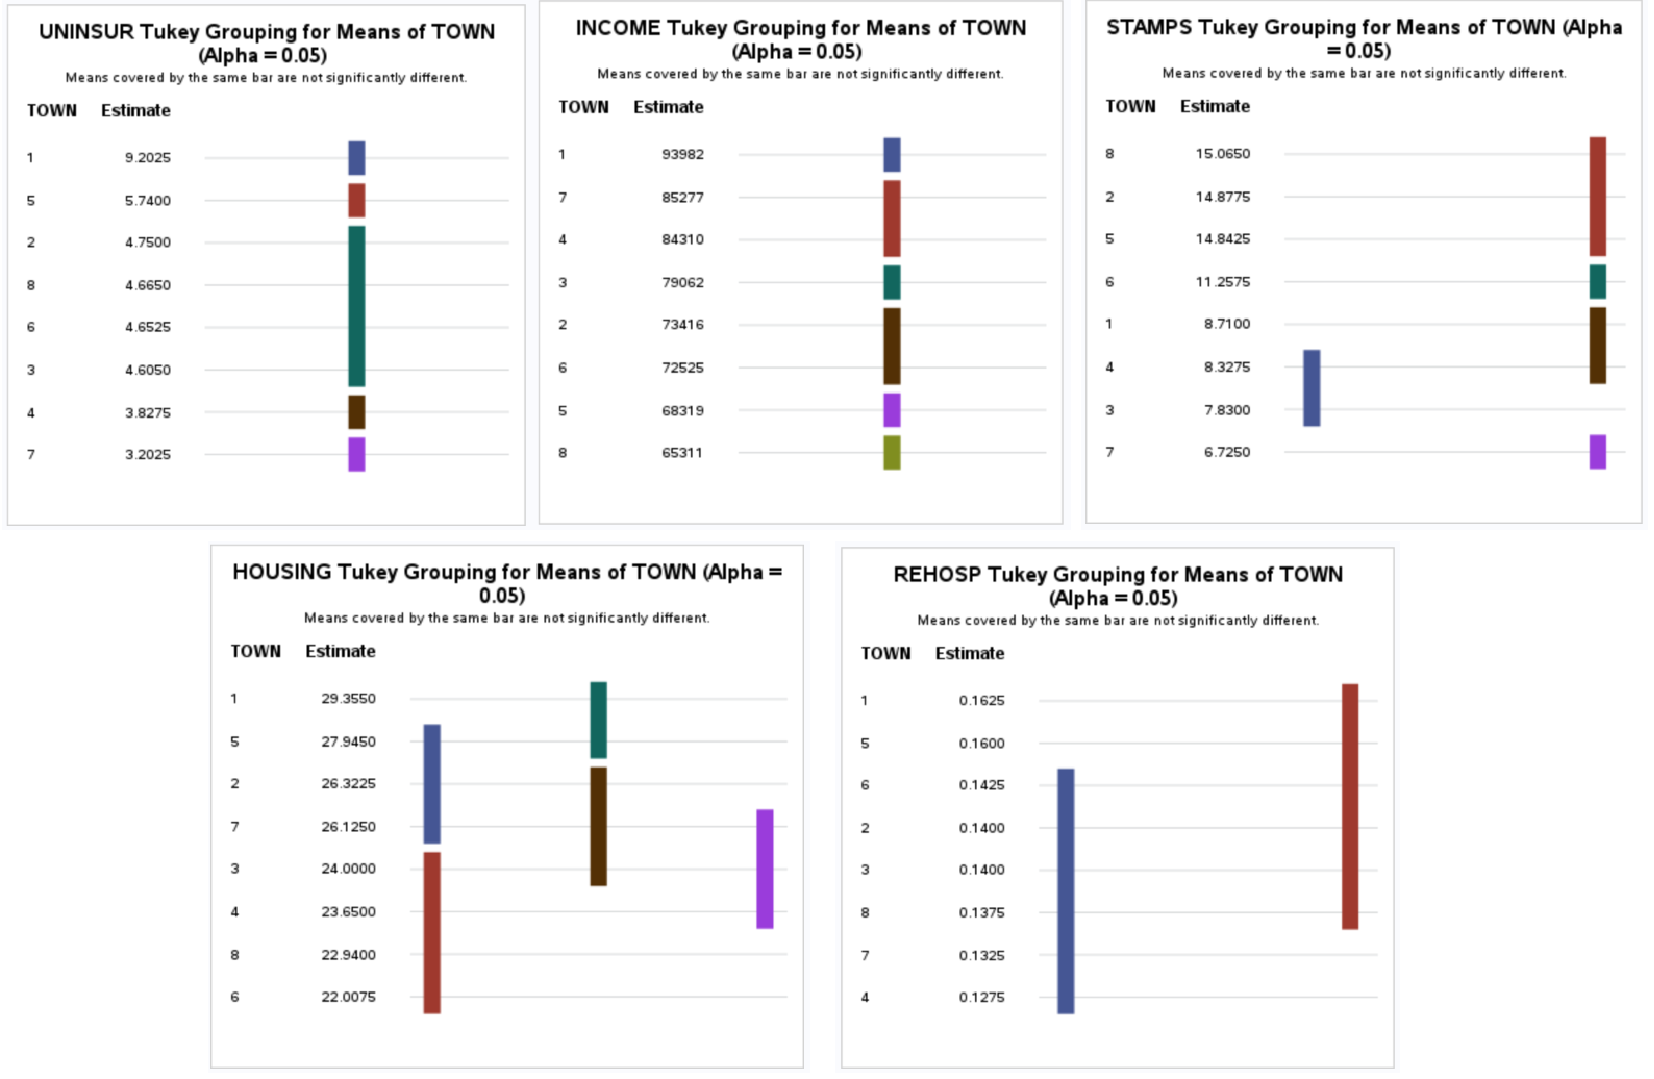
\includegraphics[width=\textwidth]{Multiple Comparisons by County.pdf}
    \caption{Social Needs Multiple Comparisons by County.}
  \end{figure}

  \begin{figure}[tbp]
    \label{fig:Social Needs by YearGraph}
      \centering
      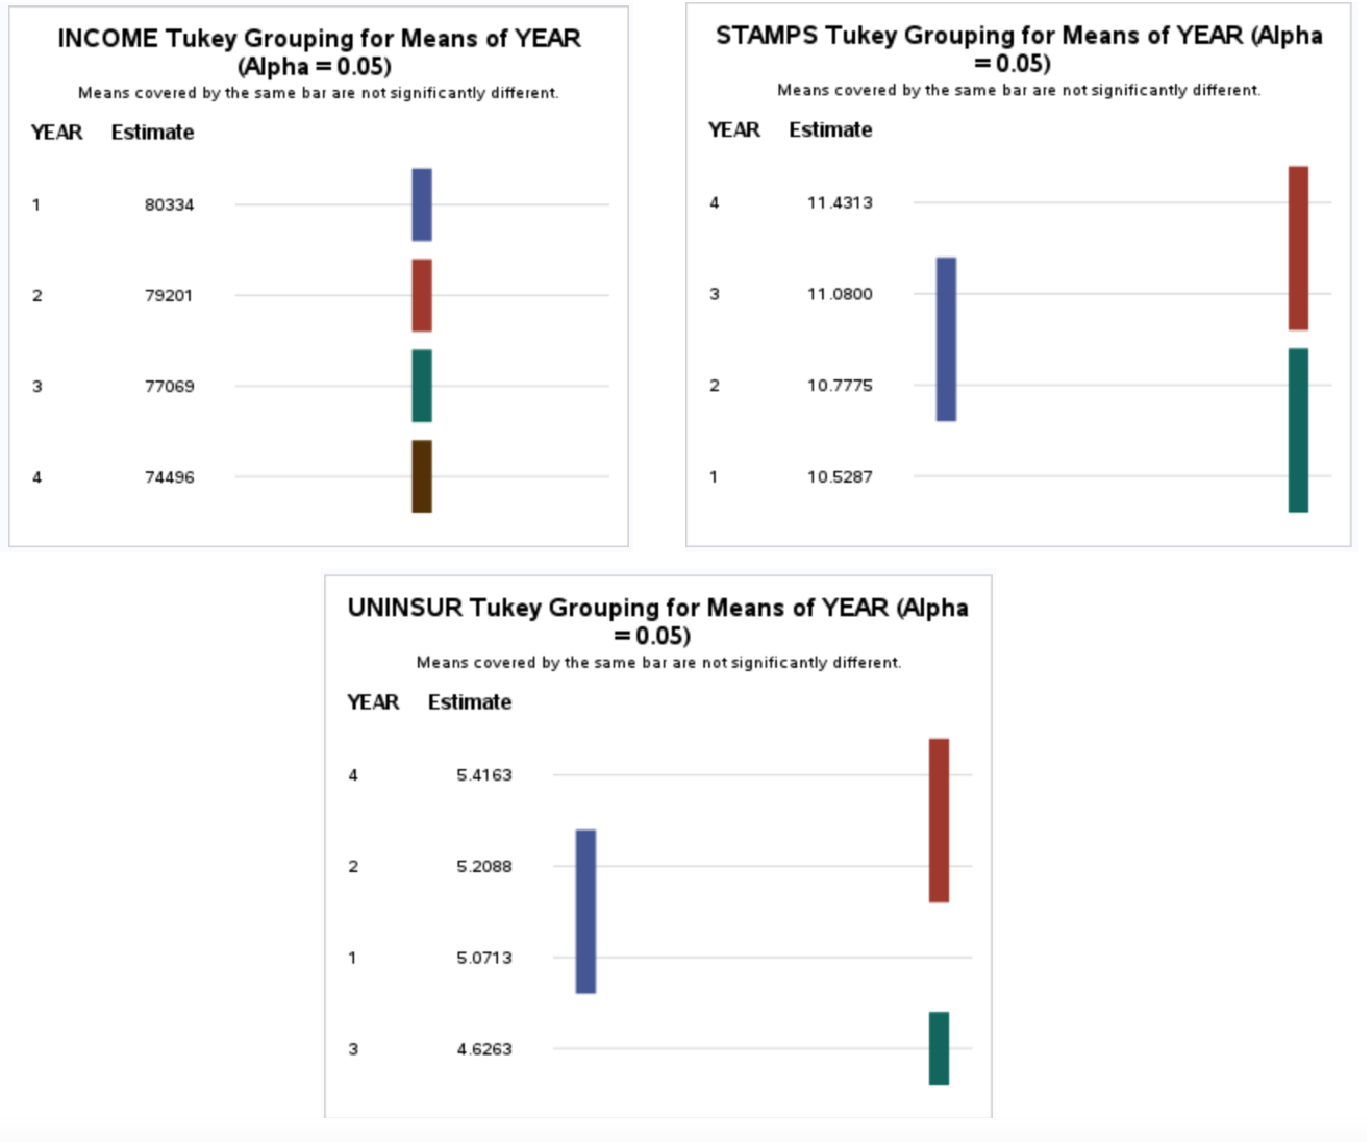
\includegraphics[width=\textwidth]{By Year.pdf}
      \caption{Social Needs Multiple Comparisons by County.}
    \end{figure}

  \begin{table}[htbp]
    \label{tab:Multiple Comparison for Income}
    \caption{Median Income Multiple Comparison by County}
    \centering
    \resizebox{\columnwidth}{!}{%
    \begin{tabular}{lllrrrr}
    \toprule
    & & & \multicolumn{1}{l}{} & \multicolumn{1}{l}{} & \multicolumn{2}{l}{95\% Confidence} \\
    County 1(I) & County 2(J) & Mean Difference(I-J) & \multicolumn{1}{l}{Std. Error} & \multicolumn{1}{l}{Sig.} & \multicolumn{1}{l}{Lower Bound} & \multicolumn{1}{l}{Upper Bound} \\
    \midrule
    Fairfield County & Hartford County & 20565.50* & 1883.47 & \textbf{\textless0.001} & 14327.60 & 26803.40 \\
    & Litchfield County & 14919.50* & 1883.47 & \textbf{\textless0.001} & 8681.60 & 21157.40 \\
    & Middlesex County & 9671.75* & 1883.47 & \textbf{\textless0.001} & 3433.85 & 15909.65 \\
    & New Haven County & 25662.75* & 1883.47 & \textbf{\textless0.001} & 19424.85 & 31900.65 \\
    & New London County & 21456.50* & 1883.47 & \textbf{\textless0.001} & 15218.60 & 27694.40 \\
    & Tolland County & 8705.00* & 1883.47 & \textbf{0.002} & 2467.10 & 14942.90 \\
    & Windham County & 28671.00* & 1883.47 & \textbf{\textless0.001} & 22433.10 & 34908.90 \\
    \midrule
    Hartford County & Fairfield County & -20565.50* & 1883.47 & \textbf{\textless0.001} & -26803.40 & -14327.60 \\
    & Litchfield County & -5646 & 1883.47 & 0.096 & -11883.90 & 591.90 \\
    & Middlesex County & -10893.75* & 1883.47 & \textbf{\textless0.001} & -17131.65 & -4655.85 \\
    & New Haven County & 5097.25 & 1883.47 & 0.169 & -1140.65 & 11335.15 \\
    & New London County & 891 & 1883.47 & 1 & -5346.90 & 7128.90 \\
    & Tolland County & -11860.50* & 1883.47 & \textbf{\textless0.001} & -18098.40 & -5622.60 \\
    & Windham County & 8105.50* & 1883.47 & \textbf{0.005} & 1867.60 & 14343.40 \\
    \midrule
    Litchfield County & Fairfield County & -14919.50* & 1883.47 & \textbf{\textless0.001} & -21157.40 & -8681.60 \\
    & Hartford County & 5646 & 1883.47 & 0.096 & -591.90 & 11883.90 \\
    & Middlesex County & -5247.75 & 1883.47 & 0.145 & -11485.65 & 990.15 \\
    & New Haven County & 10743.25* & 1883.47 & \textbf{\textless0.001} & 4505.35 & 16981.15 \\
    & New London County & 6537 & 1883.47 & 0.035 & 299.10 & 12774.90 \\
    & Tolland County & -6214.5 & 1883.47 & 0.051 & -12452.40 & 23.40 \\
    & Windham County & 13751.50* & 1883.47 & \textbf{\textless0.001} & 7513.60 & 19989.40 \\
    \midrule
    Middlesex County & Fairfield County & -9671.75* & 1883.47 & \textbf{\textless0.001} & -15909.65 & -3433.85 \\
    & Hartford County & 10893.75* & 1883.47 & \textbf{\textless0.001} & 4655.85 & 17131.65 \\
    & Litchfield County & 5247.75 & 1883.47 & 0.145 & -990.15 & 11485.65 \\
    & New Haven County & 15991.00* & 1883.47 & \textbf{\textless0.001} & 9753.10 & 22228.90 \\
    & New London County & 11784.75* & 1883.47 & \textbf{\textless0.001} & 5546.85 & 18022.65 \\
    & Tolland County & -966.75 & 1883.47 & 0.999 & -7204.65 & 5271.15 \\
    & Windham County & 18999.25* & 1883.47 & \textbf{\textless0.001} & 12761.35 & 25237.15 \\
    \midrule
    New Haven County & Fairfield County & -25662.75* & 1883.47 & \textbf{\textless0.001} & -31900.65 & -19424.85 \\
    & Hartford County & -5097.25 & 1883.47 & 0.169 & -11335.15 & 1140.65 \\
    & Litchfield County & -10743.25* & 1883.47 & \textbf{\textless0.001} & -16981.15 & -4505.35 \\
    & Middlesex County & -15991.00* & 1883.47 & \textbf{\textless0.001} & -22228.90 & -9753.10 \\
    & New London County & -4206.25 & 1883.47 & 0.368 & -10444.15 & 2031.65 \\
    & Tolland County & -16957.75* & 1883.47 & \textbf{\textless0.001} & -23195.65 & -10719.85 \\
    & Windham County & 3008.25 & 1883.47 & 0.747 & -3229.65 & 9246 \\
    \midrule
    New London County & Fairfield County & -21456.50* & 1883.47 & \textbf{\textless0.001} & -27694.40 & -15218.60 \\
    & Hartford County & -891 & 1883.47 & 1 & -7128.90 & 5346.90 \\
    & Litchfield County & -6537.00* & 1883.47 & 0.035 & -12774.90 & -299.10 \\
    & Middlesex County & -11784.75* & 1883.47 & \textbf{\textless0.001} & -18022.65 & -5546.85 \\
    & New Haven County & 4206.25 & 1883.47 & 0.368 & -2031.65 & 10444.15 \\
    & Tolland County & -12751.50* & 1883.47 & \textbf{\textless0.001} & -18989.40 & -6513.60 \\
    & Windham County & 7214.50* & 1883.47 & 0.016 & 976.60 & 13452.40 \\
    \midrule
    Tolland County & Fairfield County & -8705.00* & 1883.47 & 0.002 & -14942.90 & -2467.10 \\
    & Hartford County & 11860.50* & 1883.47 & \textbf{\textless0.001} & 5622.60 & 18098.40 \\
    & Litchfield County & 6214.50 & 1883.47 & 0.051 & -23.40 & 12452.40 \\
    & Middlesex County & 966.75 & 1883.47 & 0.999 & -5271.15 & 7204.65 \\
    & New Haven County & 16957.75* & 1883.47 & \textbf{\textless0.001} & 10719.85 & 23195.65 \\
    & New London County & 12751.50* & 1883.47 & \textbf{\textless0.001} & 6513.60 & 18989.40 \\
    & Windham County & 19966.00* & 1883.47 & \textbf{\textless0.001} & 13728.10 & 26203.90 \\
    \midrule
    Windham County & Fairfield County & -28671.00* & 1883.47 & <.001 & -34908.90 & -22433.10 \\
    & Hartford County & -8105.50* & 1883.47 & 0.005 & -14343.40 & -1867.60 \\
    & Litchfield County & -13751.50* & 1883.47 & \textbf{\textless0.001} & -19989.40 & -7513.60 \\
    & Middlesex County & -18999.25* & 1883.47 & \textbf{\textless0.001} & -25237.15 & -12761.35 \\
    & New Haven County & -3008.25 & 1883.47 & 0.747 & -9246.15 & 3229.65 \\
    & New London County & -7214.50* & 1883.47 & 0.016 & -13452.40 & -976.60 \\
    & Tolland County & -19966.00* & 1883.47 & \textbf{\textless0.001} & -26203.90 & -13728.10 \\
    \bottomrule
    * The mean difference is significant at the 0.05 level\\
  \end{tabular}%
  }
\end{table}
    
\begin{table}[]
  \label{tab: Multiple Comparisons}
  \caption{Multiple Comparisons by Year and Town}
  \resizebox{\columnwidth}{!}{%
  \begin{tabular}{llrrrrl}
  \textbf{Social Need}   & \textbf{Comparison by} & \multicolumn{1}{l}{\textbf{DF}} & \multicolumn{1}{l}{\textbf{Sum of Squares}} & \multicolumn{1}{l}{\textbf{Mean Square}} & \multicolumn{1}{l}{\textbf{F Value}} & \textbf{p Value}           \\
  Median Income          & Year                   & 3                               & 158657606                                   & 52885869                                 & 95.57                                & \textbf{\textless0.001}                    \\
                         & Town                   & 7                               & 2618521106                                  & 374074444                                & 675.99                               & \textbf{\textless0.001}                      \\
  Food                   & Year                   & 3                               & 3.6450625                                   & 1.2150208                                & 10.08                                & \textbf{0.0003} \\
                         & Town                   & 7                               & 348.3382875                                 & 49.7626125                               & 412.72                               & \textbf{\textless0.001}                      \\
  Housing                & Year                   & 3                               & 1.4535125                                   & 0.4845042                                & 0.41                                 & 0.7506 \\
                         & Town                   & 7                               & 183.9498375                                 & 26.2785482                               & 21.99                                & \textbf{\textless0.001}                      \\
  Rehospitalization Rate & Year                   & 3                               & 0.00050938                                  & 0.00016979                               & 1.45                                 & 0.2578 \\
                         & Town                   & 7                               & 0.00427188                                  & 0.00061027                               & 5.2                                  & \textbf{0.0015} \\
  Uninsured Rate         & Year                   & 3                               & 2.6848375                                   & 0.89494583                               & 17.17                                & \textbf{\textless0.001}                     \\
                         & Town                   & 7                               & 92.8554875                                  & 13.26506964                              & 254.57                               & \textbf{\textless0.001}    \\                
  * The mean difference is significant at the 0.05 level\\
  \end{tabular}%
  }
  \end{table}

\section{Discussion}\label{sec:disc}

\ref{fig:Education by County Graph}
discuss, use lit to support why(descriptive) specific to CT


Table 4\ref{fig:Social Needs by County Graph} reveals that there is a signifiant difference between 
social need variables by year (2017-2020) for median income, food, and uninsured rate. Table 4 also 
reveals that all five variables analyzes(median income, food, housing, rehospitalization rate, and 
uninsured rate) are significantly difference. Multiple Comparison tests are conducted to identify the 
specific similarities and differences between the 8 CT counties.
\\
I. Comparison by County
\\
The results of the Tukey multiple comparison analysis\ref{tab: Multiple Comparisons} shed light on the relationship between county and key 
variables such as median income, housing affordability, rehospitalization rates, food stamps usage, and
uninsured rates. Understanding these correlations is vital in comprehending 
the socio-economic and racial disparities prevalent in the studied region.

The disparity in median income over the studied years, particularly the peak observed in 2020, 
signifies economic fluctuations. Notably, county 1 stands out with significantly higher income 
compared to other counties, indicating potential disparities in resource access and opportunities. 
\ref{tab:Multiple Comparison for Income} displays the individual significant levels for comparison with County 1.
All counties 2-8 appear to be significantly different at p <0.05 compared to county 1.
This wealth gap implies potential repercussions on community health outcomes. The consistent trend in 
the percentage of income spent on rent underscores a persistent challenge for residents, especially 
noticeable in counties 1 and 5, indicating enduring economic pressure.

The results pertaining to housing defined by renters whose rent is 50 percent of their income, 
reveal noteworthy patterns with respect to social needs. Examining the data across the four-year span 
indicates a consistent trend, as no significant differences were observed. However, significant differences are 
revealed when comparing between counties. Counties 1 and 5 exhibited a statistically significant increase 
in the percentage of renters facing housing costs amounting to 50 percent of their income compared to 
counties 2, 7, and 3. Intriguingly, there was no statistically significant distinction between counties 
1 and 5, suggesting a commonality in the challenges faced by renters in these specific regions. These 
findings underscore the importance of localized interventions and policy considerations to address the 
distinct socio-economic dynamics influencing housing affordability across different counties.

Food access was assesses through investigating the proportion of the population involved in the use of Food Stamps programs.
AHRQ data reveals notable variations across different counties. Counties 8, 2, and 5 exhibit a statistically significant 
higher percentage of the population relying on Food Stamps, suggesting a potentially elevated level of economic 
vulnerability or socio-economic challenges in these areas. County 6 also demonstrates a substantial proportion 
of its population on Food Stamps, indicating a notable need for social assistance. Conversely, County 7 stands 
out with the lowest percentage of its population depending on Food Stamps, implying comparatively better 
economic conditions or potentially more effective social support systems. These findings underscore the 
importance of targeted interventions and resource allocation to address social needs, particularly in counties 
with higher reliance on Food Stamps. Further exploration into the underlying factors contributing to these variations 
is needed for informed policy development and community-specific interventions.

Rehospitalization rates demonstrate stability across counties and years leading up to 2020, suggesting 
a consistent healthcare landscape. Counties 8, 2, and 5 exhibiting higher food stamp usage point to economic 
challenges faced by residents in these regions. This trend aligns with housing affordability issues, 
indicating a correlation between financial stress and reliance on government assistance programs.

The notably high uninsured rate in county 1 raises concerns about healthcare accessibility, likely 
linked to economic factors impacting insurance affordability. Conversely, the lower uninsured rate in 
Year 3 (2019) signifies positive progress. Analyzing the policies or interventions implemented during 
this period could provide valuable insights for effective healthcare reforms, offering potential guidance 
for future initiatives.

These analyses reveals the presence of a drastic inequality in County 1(Fairfield County). Although Farfield County
is revealed to have the highest median income, greatest educational attainment, Farfield County also has the greatest 
percent population uninsured with health insurance and the greatest proportion of population whose renters pay rent 
50 percent of their income. According to a study by the Federal Reserve Bank of New York{ ???????}, the most highest paid 
workers in Fairfield County earn a salary that is nine times greater than their lower-wage counterparts. Technology causing the disparities
\\
II. Comparison by Year
\\
An analysis spanning four years indicates significant differences in median income, with the highest observed 
in 2020 and the lowest in 2017. While there doesn't seem to be a notable overall difference in the proportion 
of the population relying on food stamp programs or facing uninsured rates, distinctions emerge when considering 
specific timeframes. The use of food stamps was higher in 2020 and 2019 compared to 2017, showcasing a 
shift in reliance on such programs over the years. Similarly, the uninsured rates were notably higher in 2020 and 
2018 compared to 2019. These findings suggest despite an overall increase in income over time, there is a simultaneous 
growing demand for food stamp programs and a pressing need for improved access to affordable health insurance. 
This suggests that, while income is on the rise, significant portions of the population still face challenges in
 meeting basic needs and accessing essential services. Addressing these trends requires comprehensive strategies 
 that go beyond income growth alone.



\subsection{Limitations}
One limitation lies in the availability and quality of data. This dataset does not have any 
data from years after 2020 which may serve to limit potential external validity considerations. 
There may also be variability in data collection methods and discrepancies in reporting standards 
leading to missing or incomplete data over the course of 4 years. Another limitation involves the scope 
of the study, focusing on specific counties in Connecticut may not fully capture nationwide disparities. 
Additionally, the research is limited to the factor parameters selected to investigate which  might not 
encompass all relevant social determinants affecting health outcomes.

\subsection{Future Directions}
These findings underscore the complex interplay between socio-economic status, race, and health outcomes. 
Addressing these disparities requires multifaceted interventions, including economic support, affordable 
housing initiatives, and targeted healthcare access programs. Future research should delve deeper into the 
root causes of these disparities, considering historical and systemic factors. Additionally, policy interventions 
and community-based programs should be designed to specifically target areas and populations facing the most 
significant challenges, aiming for a more equitable healthcare landscape for all residents.


\appendix

\bibliography{../manuscript/ref}
\bibliographystyle{chicago}

\end{document}

{housing by income.pdf}
{housing by year.pdf}
{Income by town.pdf}
{Inome by year.pdf}
{Rehosp by income/year.pdf}
{Stamps by income/year.pdf}